\documentclass[11pt]{article}
\usepackage{amsmath,amssymb,amsthm}
\usepackage[shortlabels]{enumitem}
\usepackage{tabu}
\usepackage{graphicx}
%\usepackage[bw]{mcode}
\usepackage[margin=.6in]{geometry}
\usepackage{tikz}
\usepackage{float}
\usepackage{textcomp}
\usepackage{multicol}
\addtolength{\topmargin}{.5in}
\usepackage{fancyhdr}
\usetikzlibrary{positioning}
\usepackage{pgfplots}
\usepackage{enumitem}
\usepackage{xcolor}
\usepackage{caption}
\setlength{\parindent}{0pt}
\setlength{\parskip}{5pt plus 1pt}
\setlength{\headheight}{20pt}
\renewcommand{\headrulewidth}{0pt}
\setlength{\headheight}{30.0pt}
\newcommand\question[2]{\vspace{.25in}\hrule\textbf{#1: #2}\vspace{.5em}\hrule\vspace{.10in}}
\renewcommand\part[1]{\vspace{.10in}\textbf{(#1)}}
\newcommand\enter{\vspace{.50in}}
\newcommand\algorithm{\vspace{.10in}\textbf{Algorithm:}}
\newcommand\correctness{\vspace{.10in}\textbf{Correctness: }}
\newcommand\runtime{\vspace{.10in}\textbf{Running time: }}
\pagestyle{fancyplain}

\begin{document}\raggedright
\newcommand\Page{\page  / \lastPage}
\newcommand\page{1}
\newcommand\qN[2]{\Large {#1} \small{#2} \normalsize}

% info
\newcommand\dueDate{\today}
\newcommand\hwnum{6}
\newcommand\ExNum{}

\newcommand\lastPage{3}

% set info

\chead{\LARGE{\textbf{CAPSTONE PROJECT INSTRUCTIONS}\\ \color{red}Rubric}}
\centering
\textbf{Due Dec 3, 2021}\\
\hrulefill
\flushleft
\vspace{1cm}
The components of the final project are as follows:
\begin{itemize}
	\item The following items are due on \textbf{December 3} by \textbf{11:59 pm}
	\begin{itemize}
		\item You must complete sections 1-3 outlined below. Any code written must be well commented.
		\item You must submit your full SciProgLib library containing all codes completed during lecture and any additional programs written for this project. See details in section 4.
		\item A written report, 12pt font, double spaced. This report should contain your responses to question prompts and figures where necessary.		
	\end{itemize}
\end{itemize}

\begin{table}[H]
	\centering
	\color{red}
	\begin{tabular}{| c | c| c | c|}
		\hline
		Question & Part & Score & Total Points \\
		\hline
		1 (30pts total) & a & & 9pts \\
		                & b & & 6pts \\
		                & c & & 15pts \\
		\hline
		2 (30pts total) & a & & 13pts \\
						& b & & 4pts \\
						& c & & 13pts \\
		\hline
		3 (30pts total) & a & & 14pts \\
						& b & & 12pts \\
						& c & & 4pts \\
	   \hline
	   4 (10pts total) & -- & &  10pts\\
	   \hline
	\end{tabular}
\end{table}
\centering \color{white} 1000000000000000000 \color{red}\textbf{Total Score} \color{white} 100 \color{red} \textbf{/100} \color{black}

\newpage
%%%%%%%%%%%%%%%%%%%%%%%%%%%%%%%%%%%%%%%%%%%%%%%%%%%%%%%%%%%%%%%%%%%%%%%%%%%%%%%%%%%%%%%%%%%%%%
\question{1}{Root Finding Methods \color{red} 30pts}
\begin{enumerate}[(a)]
	\item \textbf{Secant Method \color{red} 9pts}\\
	A potential problem in implementing the Newton-Raphson method is
	the evaluation of the derivative. Although this is not inconvenient for polynomials and many other functions, there are certain functions whose derivatives may be difficult or inconvenient to evaluate. For these cases, the derivative can be approximated by a backward finite divided difference:
	$$ f'(x_i) \approx \frac{f(x_{i})-f(x_{i-1})}{x_{i}-x_{i-1}}$$
	and substitute it into our Newton-Raphson formula
	$$x_{i+1} = x_i - \frac{f(x_i)}{f'(x_i)}$$
	we end up with 
	$$x_{i+1} = x_i - \frac{f(x_i)\left(x_{i}-x_{i-1}\right)}{f(x_{i})-f(x_{i-1})} $$
	This is the formula for a \textit{Secant method}. Notice that the approach requires two initial estimates of $x$. However, because $f(x)$ is not required to change signs between the estimates, it is not classified as a bracketing method. \\\vspace{10pt}
	Write a function that implements the secant method. Use the function name and parameters specified below. \textbf{Use one of your differentiation codes to approximate the derivative.} \\\vspace{10pt}
	\texttt{Secant(double x0, double x1, double tol, int Maxit, double(*f)(double x))}
	\begin{table}[H]
		\centering
		\color{red}
		\begin{tabular}{| c | l |}
			\hline
			Points & \\
			\hline
			9 & Code compiles and is well commented. \\
			\hline
			7 & Code compiles, but is not well commented. \\
			\hline
			5 & Code compiles, but does not call a differentiation method. \\
			  & Code does not compile, but errors are small. \\
			\hline
			0 & Code does not compile, errors are significant.\\
			\hline
		\end{tabular}
	\end{table}
	\item \textbf{Secant Method Test \color{red} 6pts}\\
	Use your \texttt{Secant} code to determine the \underline{mass} of the bungee jumper with a drag coefficient of 0.25 kg/m to have a velocity of 36 m/s after 4 s of free fall. The acceleration of gravity is 9.81 m/$\textrm{s}^2$. Use initial guesses of 40 kg and 50 kg and tol = 0.0001.\\ 
	\vspace{5pt}
	\textbf{Report:}
	\begin{itemize}
		\item the mass of the bungee jumper
		\item iterations it needed to find the root of the function
	\end{itemize}
	Do the same experiment using your \texttt{Bisect} and \texttt{NewtonRaphson} codes. For \texttt{Bisect}, use an initial guess of 40 kg and 250 kg. For \texttt{NewtonRaphson}, use an initial guess of 50 kg. \textbf{Compare} the results of the three methods. Recall, the function for the bungee jumper is
	$$f(m) = \sqrt{\frac{gm}{c_d}}\tanh\left(t\sqrt{\frac{gc_d}{m}}\right) -v(t), $$
	\newpage
	with the derivative
	$$f'(m) = \frac{1}{2}\sqrt{\frac{g}{mc_d}}\tanh\left(t\sqrt{\frac{gc_d}{m}}\right) - \frac{gt}{2m}\left(1-\tanh^2\left(t\sqrt{\frac{gc_d}{m}}\right)\right). $$ 
	\begin{table}[H]
		\centering
		\color{red}
		\begin{tabular}{| l | l | c | c | c | c | c |}
			\hline
			Method &  & Mass & Iterations & Correct & Incorrect due to & Not submitted\\
			       &  &      &            &                  &  small logic error & Incorrect due to \\
			       &  &      &            &                  &                    & major logic error \\
			\hline
			Secant & Backward Difference & 142.7329 & 6 & & &\\
			              & Forward Difference & 142.7329 & 6 & 2pts & 1pts & 0pts\\
			              & Centered Difference &142.7376 & 8 & & &\\
			\hline
			Newton-Raphson & & 142.7376 & 5 & 2pts & 1pts & 0pts\\
			\hline
			Bisection & & 142.7313 & 14 & 2pts & 1pts & 0pts\\
			\hline
		\end{tabular}
	\end{table}
\end{enumerate}
\begin{enumerate}[(c)]
	\item \textbf{Case Study - Newton-Raphson and the Bisection Method \color{red} 15pts}\\
	Determine the positive root of $$f(x) = x^{10} - 1$$ using the 
	\begin{itemize}
		\item Newton-Raphson method and an initial guess of $x = 0.5$ and tol = 0.0001.
		\item Bisection method with an initial guess of $a = 0.5$, and $b = 1.1$, and tol = 0.0001.
	\end{itemize}
    The derivative of $f(x)$ is $$f'(x) = 10x^9.$$
   
	\textbf{Report:}
	\begin{itemize}
		\item the root for each method \color{red} 1pt per method, 2pts total \color{black}
		\item the number of iterations it took each method to find the root \color{red} 1pt per method, 2pts total
	\end{itemize}
	\textbf{Compare} your results. Sketch the first few iterations of the Newton-Raphson method \color{red}(5pts) \color{black}to explain your results \color{red}(6pts).
	\begin{table}[H]
		\centering
		\color{red}
		\begin{tabular}{| l | c | c | c | c | c |}
			\hline
			Method & Root & Iterations & Correct & Incorrect due to & Not submitted\\
			&        &            &                  &  small logic error & Incorrect due to \\
			&        &            &                  &                    & major logic error \\
			\hline
			Newton-Raphson  & 1.0000239 & 42 & 2pts & 1pts & 0pts\\
			\hline
			Bisection &  1.0000244 & 13 & 2pts & 1pts & 0pts\\
			\hline
		\end{tabular}
	\end{table}
	\color{red} The bisection method converges quicker than Newton-Raphson even though it is a bracketing method. This is because of our initial guess for the method. At this point, the slope of the curve is very close to 0 which yields a much larger guess for $x_1$, since $x_1$ is the point where the tangent curve passes through the x-axis. We see the subsequent values of $x$ decrease, meaning that it is converging to our solution. Because of this, it takes several iterations for the Newton-Raphson method to converge to the root. (6pts full response, 3pts partial response, 0pts no response)
	\begin{figure}[H]
		\centering
		\includegraphics[width = .7\textwidth]{1cplot}
		\caption*{\color{red} 5pts figure contains $x_0$, initial tangent curve, and itentifies at least 2 more points. \\
		3pts figure contains $x_0$ and initial tangent curve but does not identify any future points. \\
	    1pt figure only contains $x_0$. \\
        0pts Incorrect response.}
	
	
	\end{figure}
\end{enumerate}
 
\newpage
%%%%%%%%%%%%%%%%%%%%%%%%%%%%%%%%%%%%%%%%%%%%%%%%%%%%%%%%%%%%%%%%%%%%%%%%%%%%%%%%%%%%%%%%%%%%%%
\question{2}{Optimization \color{red} 30pts}
\begin{enumerate}[(a)]
	\item \textbf{Golden-Section Search \color{red} 13pts}\\
	Your current \texttt{GoldenSectionSearch} code only finds the minimum values of a function. \textbf{Explain} why \color{red} (3pts) \color{black} and \textbf{modify} your function so that it takes in a boolean as an input \color{red}(10pts)\color{black}, i.e.\\ \texttt{GoldenSectionSearch(double xl, double xu, double tol, double (*f)(double x), bool min)}  
	\begin{itemize}
		\item if \texttt{min} is \texttt{true}, your function should return the minimum of the function.
		\item if \texttt{min} is \texttt{false}, your function should return the maximum of the function.
	\end{itemize}
	\color{red}The Golden-Section search compares $f(x_i)$ and $f(x_{i+1})$ and looks for the smaller value. This allows the method to specifically converge to the minimum value. If we want the method to look for a maximum, we would need to compare these two values and look for the larger value. (3pts correct response, 2pts partially correct response, 0pts incorrect/no resonse.)
	
	\begin{table}[H]
		\centering
		\color{red}
		\begin{tabular}{| c | l |}
			\hline
			Points & \\
			\hline
			10 & Code compiles and is well commented. \\
			\hline
			8 & Code compiles, but is not well commented. \\
			\hline
			5 & Code does not compile, but errors are small. \\
			\hline
			0 & Code does not compile, errors are significant. \\
			  & Code compiles but does not address the question.\\
			  \hline
		\end{tabular}
	\end{table}
	\color{black}
	\item \textbf{Golden-Section Search Test \color{red} 4pts}\\
	Use your function \texttt{GoldenSectionSearch} to find the 
	\begin{itemize}
		\item minimum using $x_l = 0$ and $x_u = 2\pi$ \color{red}(2pts)\color{black}
		\item maximum using $x_l = 0$ and $x_u = 2\pi$ \color{red}(2pts)\color{black}
	\end{itemize}
	of the function $f(x) = \sin(x)$.
	
	\begin{table}[H]
		\centering
		\color{red}
		\begin{tabular}{| l | c | c | c | c |}
			\hline
			 & Optima value &  Correct & Incorrect due to & Not submitted\\
			        &            &                  &  small logic error & Incorrect due to \\
			        &            &                  &                    & major logic error \\
			\hline
			Maximum  &  4.7119887 &  2pts & 1pts & 0pts\\
			\hline
			Minimum &   1.5708417 & 2pts & 1pts & 0pts\\
			\hline
		\end{tabular}
	\end{table}

	\item \textbf{The optima is 0 \color{red} 13pts}\\
	Currently, the \texttt{ParabolicInterpolation} method will not return the optima for the following function
	 $$f(x) =  -x^5 +2x^2+1$$
	 with the initial guesses $x_1 = -0.7$, $x_2=0.5$, and $x_3= 1$.
	\begin{itemize}
		\item \textbf{Explain} why. \color{red}(2pts) \color{black}
		\item \textbf{Modify} the method to address all instances of where the issue could occur so that it returns where the optima where $x\approx0$. \color{red}(7pts) \color{black}
		\item \textbf{Modify} the \texttt{GoldenSectionSearch} method to address the same type of issue. \color{red}(4pts) \color{black}
	\end{itemize}
	\newpage
	\color{red} This method breaks down when $x\approx 0$ because the denominator becomes 0. To avoid this, we can divide by the smallest machine value. (2pts complete response, 1pt incomplete response, 0pts incorrect/no response)
	
	\begin{table}[H]
		\centering
		\color{red}
		\begin{tabular}{| l | c | c | c |}
			\hline
			& Optima value &  Correct & Incorrect/Not submitted\\
			\hline
			Parabolic interpolation  & 0.00000000088569751 & 1pt & 0pts\\
			\hline
			Golden Section search    & 0.00000000745005601 & 1pt & 0pts\\
			\hline
		\end{tabular}
		\begin{table}[H]
		\centering
		\color{red}
		\begin{tabular}{| c | l | l |}
			\hline
			Points Parabolic & Points GS Search &\\
			\hline
			6 & 3 & Code compiles and is well commented. \\
			\hline
			4 & 2 & Code compiles, but is not well commented. \\
			\hline
			2 &  1 & Code does not compile, but errors are small. \\
			\hline
			0 & 0 & Code does not compile, errors are significant. \\
			& & Code compiles but does not address the question.\\
			\hline
		\end{tabular}
	\end{table}
	\end{table}
	
\end{enumerate}

%%%%%%%%%%%%%%%%%%%%%%%%%%%%%%%%%%%%%%%%%%%%%%%%%%%%%%%%%%%%%%%%%%%%%%%%%%%%%%%%%%%%%%%%%%%%%%
\question{3}{Integration \color{red}30pts}
\begin{enumerate}[(a)]
	\item \textbf{Gauss Quadrature \color{red}(14pts)}\\
	In addition to the methods we covered in class, we can also use the Gauss-Legendre formula (Gauss quadrature for short) to help us evaluate an integral. The objective of Gauss quadrature is to determine the unknown coefficients $c_0,...,c_{n-1}$ and x-values $x_0,...,x_{n-1}$ in the equation below 
	$$I \cong c_0f(x_0)+..+c_{n-1}f(x_{n-1}),$$
	where $n$ is the number of Gauss-Legendre points used to approximate the integral. These values are derived analytically on the interval $[-1,1]$, and have been summarized in the table below.
	\begin{figure}[H]
		\centering
		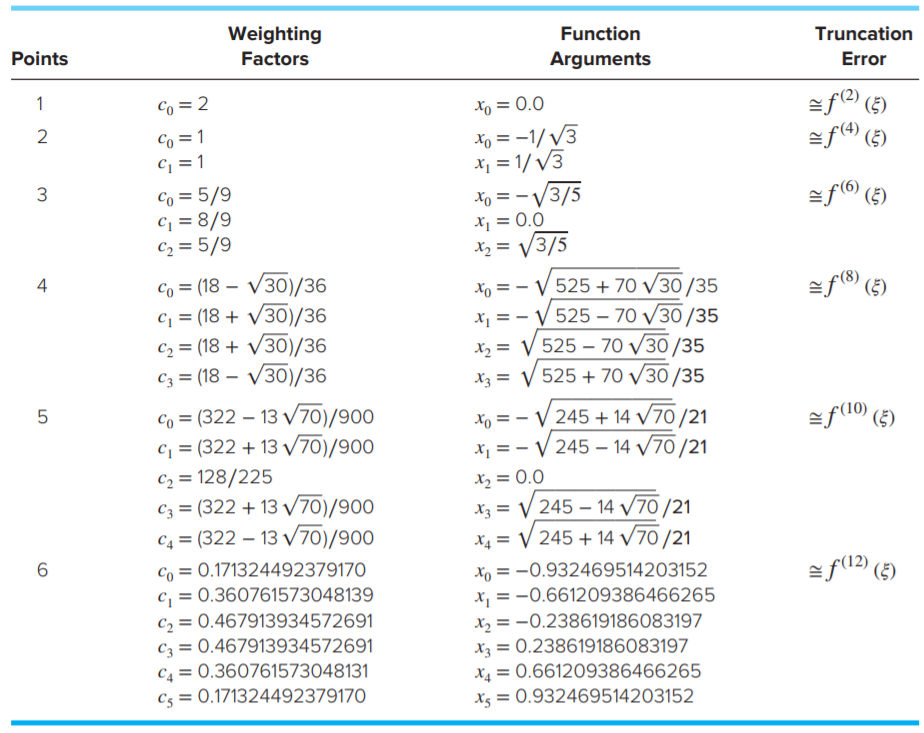
\includegraphics[width=.8\textwidth]{Integration}
	\end{figure}
	Write a function \texttt{GaussLegendre} that takes as an input
	\begin{itemize}
		\item the number of Gauss-Legendre points to be used, $n$ 
		\item a pointer to the function $f$
	\end{itemize}
	\texttt{GaussLegendre(int n, double (*f)(double(x)))}\\
	Your function should \textbf{Return} the integral approximate, $I$.
		\begin{table}[H]
		\centering
		\color{red}
		\begin{tabular}{| c | l |}
			\hline
			Points & \\
			\hline
			14 & Code compiles and is well commented. \\
			\hline
			12 & Code compiles, but is not well commented. \\
			\hline
			7 & Code does not compile, but errors are small. \\
			\hline
			0 & Code does not compile, errors are significant. \\
			& Code compiles but does not address the question.\\
			\hline
		\end{tabular}
	\end{table}
	
\end{enumerate}
\newpage
\begin{enumerate}[(b)]
	\item \color{red}(12pts) \color{black}Test your code using the function
	$$f(y) =  0.2+25y-200y^2+675y^3-900y^4+400y^5$$
	between the limits $y=0$ to $0.8$. The exact value of the integral is $1.640533333333341$ .\\\vspace{10pt}
	NOTE: Before we can approximate this function, we have to perform a change in variable so that the limits are from -1 to 1. To do this, we substitute $a = 0$ and $b= 0.8$ into the equation
	$$ y = \frac{(b+a)+(b-a)x}{2} =0.4-0.4x$$
	and 
	$$ dy = \frac{b-a}{2}dx = 0.4dx$$
	Our equation becomes
	$$f(x) = 0.4 \bigg(0.2+25(0.4-0.4x)-200(0.4-0.4x)^2+675(0.4-0.4x)^3-900(0.4-0.4x)^4+400(0.4-0.4x)^5\bigg)$$ 
	Using your code, fill in the table below.
	
	\begin{table}[H]
		\centering
		\color{red}
		\begin{tabular}{|c | c| c| c| c|}
			\hline
			n & I & \% relative error &  Correct & Incorrect/Not submitted \\
			\hline
			1 &\color{red}1.96480000000000032& \color{red}19.76592977893314540\% &1.5pts/0.5pts, 2pts tot &0pts  \\
			2 &\color{red}1.82257777777777719& \color{red}11.09666233203239116\% &1.5pts/0.5pts, 2pts tot&0pts \\
			3 &\color{red}1.64053333333332896& \color{red}0.00000000000073088\% &1.5pts/0.5pts, 2pts tot&0pts \\
			4 &\color{red}1.64053333333333073& \color{red}0.00000000000062261\% &1.5pts/0.5pts, 2pts tot&0pts \\
			5 &\color{red}1.64053333333332985& \color{red}0.00000000000067675\% &1.5pts/0.5pts, 2pts tot&0pts \\
			6 &\color{red}1.64053333333333007& \color{red}0.00000000000066321\% &1.5pts/0.5pts, 2pts tot&0pts \\
			\hline
		\end{tabular}
	\end{table}
\end{enumerate}
\begin{enumerate}[(c)]
	\item \color{red}(4pts) \color{black} How might you modify your code to compute the integral to a desired tolerance?
	
	\color{red}There are several ways to approach this question: \\
	As long as the student demonstrates good logic (4pts).\\
	If student's logic is slightly flawed (3pts). \\
	If student's logic is significantly flawed (1pt).\\
	Student did not attempt to answer the question (0pts). \color{black}
\end{enumerate}
	

\newpage
%%%%%%%%%%%%%%%%%%%%%%%%%%%%%%%%%%%%%%%%%%%%%%%%%%%%%%%%%%%%%%%%%%%%%%%%%%%%%%%%%%%%%%%%%%%%%%
\question{4}{Your Library \color{red} 10pts}
Your final library containing ALL codes listed below. Your function declarations should be identical to the ones listed below. This includes the \textbf{function name}, the \textbf{number of parameters}, and the\textbf{ order of parameters.} \\
\color{red}Deduct 1pt per function that fails the unit test \\(0.5 incorrect name/parameter list, 0.5 incorrect answer) up to 10 pts. \color{black}
\begin{itemize}
	\item The Bisection method, \\\texttt{Bisect(double a, double b, double tol, double (*f)(double x))}
	\item Newton-Raphson method, \\\texttt{NewtonRaphson(double a, double tol, int maxit, double (*f)(double x), double (*df)(double x))}
	\item Golden-Section Search Method, \\\texttt{GoldenSectionSearch(double xl, double xu, double tol, double (*f)(double x), bool min)}
	\item Parabolic Interpolation, \\\texttt{ParabolicInterpolation(double x1, double x2, double x3, double tol, double (*f)(double x))}
	\item The Recursive Trapezoid Rule for functions, \\\texttt{CompositeTrapezoid(double a, double b, int n, double avgdf2, double tol, double (*f)(double x))}
	\item Recursive Simpson's 1/3 Rule for functions, \\\texttt{CompositeSimpsons13(double a, double b, int n, double avgdf4, double tol, double (*f)(double x))}
	\item Simpson's Rules for data, \\\texttt{DataSimpsons(double x[], double fx[], int n)}
	\item Trapezoid Rule for data, \\\texttt{DataTrapezoid(vector<double> x, vector<double> fx, int n)}
	\item The Secant method \\\texttt{Secant(double x0, double x1, double tol, int maxit, double(*f)(double x))}
	\item Gauss Quadrature \\\texttt{GaussLegendre(int n, double (*f)(double(x)))}
	\item Forward finite difference \\\texttt{ForwardDifference(double x, double h, double (*f)(double x)}
\end{itemize}
\newpage
\begin{itemize}
	\item Backward finite difference \\\texttt{BackwardDifference(double x, double h, double (*f)(double x))}
	\item Centered finite difference \\\texttt{CenteredDifference(double x, double h, double (*f)(double x))}
\end{itemize}

\end{document}
